%=========================================================
\begin{figure*}[t]
\centering
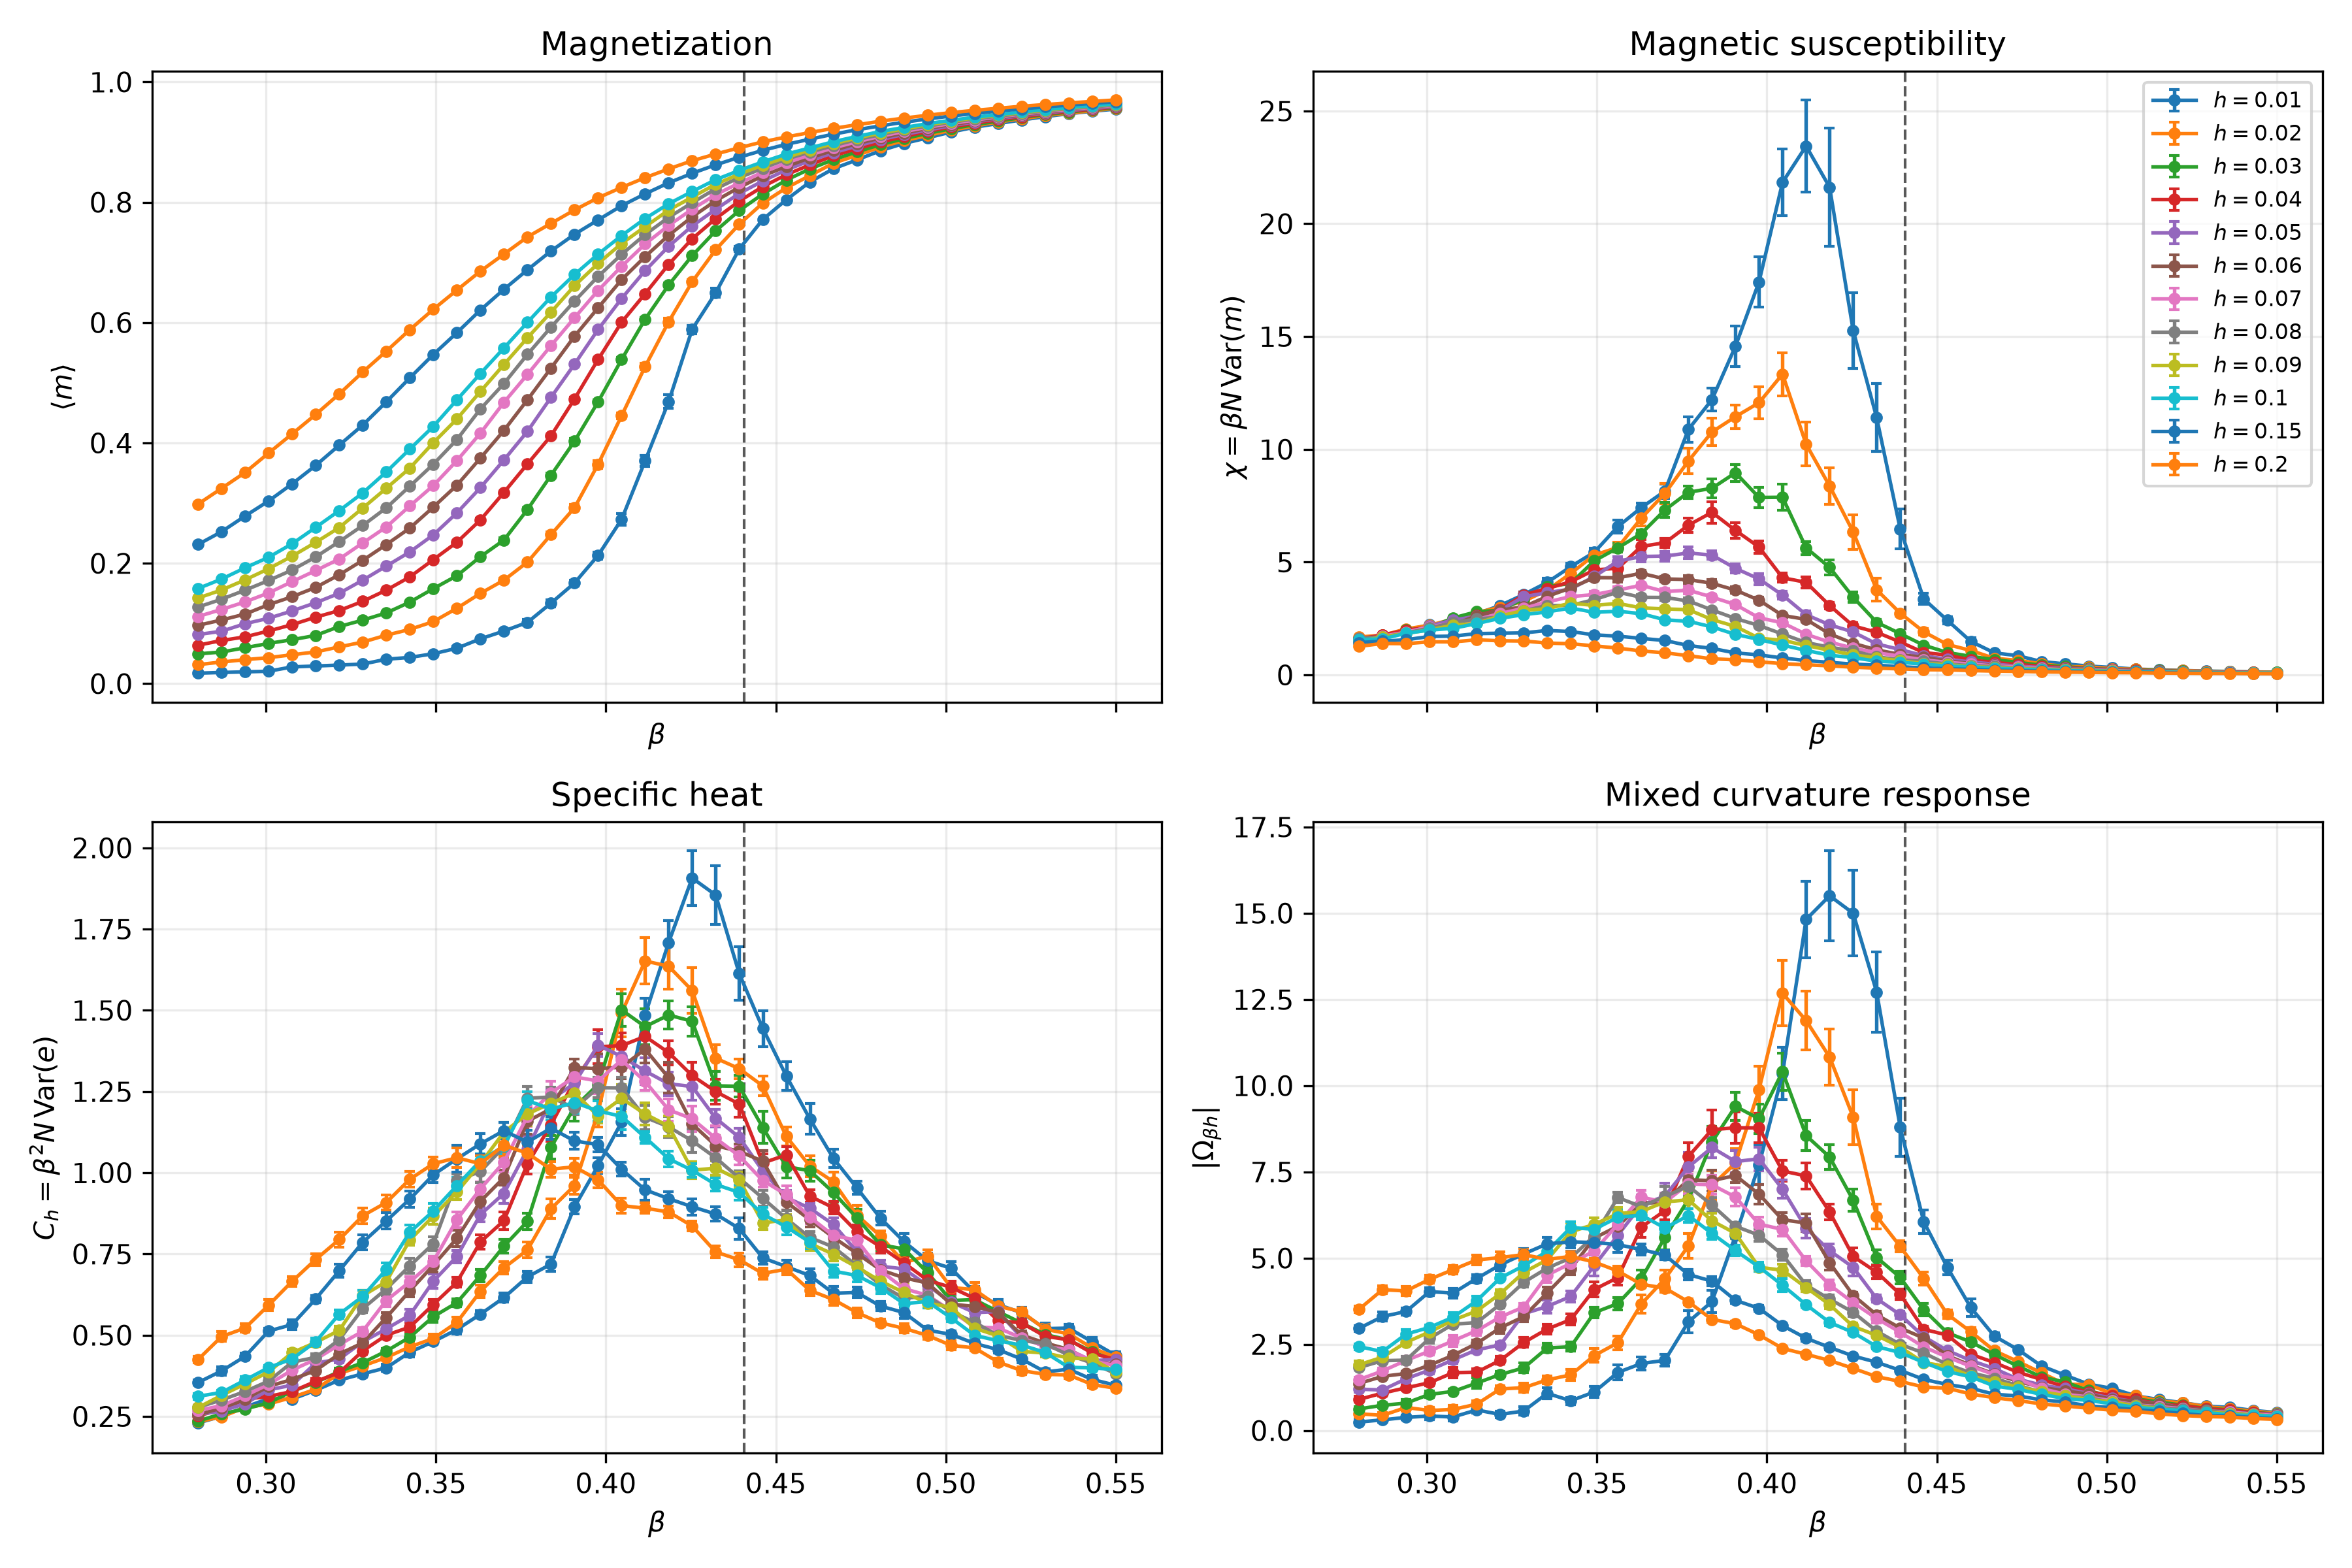
\includegraphics[width=\textwidth]{Figures/ising_cross_sections_all.png}
\caption{
Thermodynamic response functions of the two-dimensional Ising
model as functions of inverse temperature for several values
of the external magnetic field.
(a) Magnetization (m),
(b) magnetic susceptibility (\chi_T),
(c) heat capacity (C_h),
and
(d) mixed response
\(\Omega_{Th}=-\langle \delta E\delta M\rangle/(k_B T^2)\).
The first three panels represent the conventional response
functions associated with the diagonal elements of the
thermodynamic covariance matrix. The mixed response shown in
panel (d) arises from the off-diagonal covariance between
energy and magnetization fluctuations and therefore measures
the coupling between thermal and magnetic response sectors.
While all response functions exhibit enhanced behavior near the
critical region, the mixed response provides additional
information regarding the organization of correlated
fluctuations and serves as the fundamental quantity underlying
the response-geometric framework developed in this review.
}
\label{fig:ising_response_functions}
\end{figure*}
%=========================================================
